\graphicspath{{Chapter2/Figs/}}

\section{Model description} \label{mofa:model_description}

\subsection{Mathematical formulation}

Multi-Omics Factor Analysis (MOFA) is a multi-view generalisation of traditional Factor Analysis to $M$ input matrices (or views) based on the framework of Group Factor Analysis (discussed in \Cref{section:gfa}).\\
The input data consists of $M$ views $\bfY^m \in \R^{N \times D_m}$ with non-overlapping features that often represent different assays. However, there is flexibility in the definition of views.\\
Formally, the input data is factorised as:
\begin{equation} \label{mofa_master_equation}
	\mathbf{Y}^m = \mathbf{Z}(\mathbf{W}^{m}){T} + \bepsilon^m
\end{equation}
where $\bfZ \in \R^{N \times K}$ is a matrix that contains the factor values and $\bfW^m \in \R^{D_m \times K}$ are a set of $M$ matrices (one per view) that contain the weights that relate the high-dimensional space to the low-dimensional latent representation. Finally, $\bepsilon^m \in \R^{D_m}$ captures the residuals, or the noise, which is assumed to be normally distributed and heteroskedastic:
\begin{equation}
	p(\epsilon^{m}_{d}) = \Ndist{\epsilon^{m}_{d}}{0,1/\tau_{d}^{m}}
\end{equation}
where $\tau$ corresponds to the precision (inverse of the variance). Altogether, this results in the following likelihood:
\begin{equation}
	p(\bfY|\bfW,\bfZ,\bTau) = \prod_{m=1}^{M} \prod_{d=1}^{D_m} \prod_{n=1}^{N} \Ndist{y_{nd}^m}{\bfz_{n}^T\bfw_{d}^{m},(\tau_d^m)^{-1}}
	% p(y_{nd}^m) = \Ndist{y_{nd}^m}{\bfz_{n,:}\bfw_{d,:}^{mT},1/\tau_d^m},
\end{equation}

Non-Gaussian noise models can also be defined (see \Cref{section:mofa_ngaussian}), but unless otherwise stated, I will always assume Gaussian residuals.

\subsubsection{Prior distributions for the factors}  \label{section:mofa_factors}

For the factors, we can define an isotropic Gaussian prior, as commonly done in most factor analysis models:
\begin{equation}
	p(z_{nk}) = \Ndist{z_{nk}}{0,1}
\end{equation}
This effectively  assumes (1) a continuous latent space and (2) independence between samples and factors. 

\subsubsection{Prior distributions for the weights}  \label{section:mofa_weights}

The key determinant of the model is the regularization used on the prior distributions for the weights. Here we encode two levels of sparsity, a (1) view- and factor-wise sparsity and (2) an individual feature-wise sparsity. The aim of the factor- and view-wise sparsity is to disentangle the activity of factors to the different views, such that the weight vector $\bfw_{:,k}^m$ is shrunk to zero if the factor $k$ does not explain any variation in view $m$. \\
In addition, we place a second layer of sparsity which encourages inactive weights on each individual feature. Mathematically, we express this as a combination of an Automatic Relevance Determination (ARD) prior \cite{Mackay1996} for the view- and factor-wise sparsity and a spike-and-slab prior \cite{Mitchell1988} for the feature-wise sparsity:
% \begin{equation*}
% 	p(w_{dk}^{m}) = (1-\theta_{k}^{m}) \mathds{1}_0(w_{dk}^{m}) + \theta_{k}^{m} \Ndist{w_{dk}^{m}}{0, 1 / \alpha_{k}^{m}}
% \end{equation*}
However, this formulation of the spike-and-slab prior contains a Dirac delta function, which makes the inference procedure troublesome. To solve this we introduce a re-parametrization of the weights $w$ as a product of a Gaussian random variable $\hat{w}$ and a Bernoulli random variable $s$, \cite{Titsias2011} resulting in the following prior:
\begin{equation}
	p(\hat{w}_{dk}^{m},s_{dk}^{m}) = \Ndist{\hat{w}_{dk}^{m}}{0, \frac{1}{\alpha_k^m}}  \text{Ber}(s_{dk}^m \,|\,\theta_k^m)
\end{equation}
In this formulation $\alpha_k^m$ controls the activity of factor $k$ in view $m$ and $\theta_k^m$ controls the corresponding fraction of active weights (i.e. the sparsity levels).\\

Finally, we define conjugate priors for $\theta$ and $\alpha$:
\begin{align}
	p(\theta_k^m) &= \Bdist{\theta_k^m}{a_0^\theta,b_0^\theta}\\
	p(\alpha_k^m) &= \Gdist{\alpha_k^m}{a_0^\alpha, b_0^\alpha}
\end{align}
with hyper-parameters $a_0^\theta,b_0^\theta =1$ and $a_0^\alpha, b_0^\alpha=1e^{-5}$ to get uninformative priors. Posterior values of $\theta_k^m$ close to $0$ implies that most of the weights of factor $k$ in view $m$ are shrunk to $0$ (sparse factor). In contrast, a value of $\theta_k^m$ close to $1$ implies that most of the weights are non-zero (non-sparse factor). A small value of $\alpha_k^m$ implies that factor $k$ is active in view $m$. In contrast, a large value of $\alpha_k^m$ implies that factor $k$ is inactive in view $m$.

All together, the joint probability density function of the model is given by
\begin{align}
	\begin{split}
	p(\bfY,\hat{\bfW},\bfS,\bfZ,\btheta, \balpha, \btau)  = &\prod_{m=1}^{M} \prod_{n=1}^{N} \prod_{d=1}^{D_m} \Ndist{y_{nd}^m}{\sum_{k=1}^{K} s_{dk}^m \hat{w}_{dk}^m z_{nk},1/\tau_d} \\
	& \prod_{m=1}^{M}\prod_{d=1}^{D_m} \prod_{k=1}^{K} \Ndist{\hat{w}_{dk}^m}{0,1/\alpha_k^m} \text{Ber}(s_{d,k}^m|\theta_k^m) \\
	& \prod_{n=1}^{N} \prod_{k=1}^{K} \Ndist{z_{nk}}{0,1} \\
	& \prod_{m=1}^{M} \prod_{k=1}^{K} \Bdist{\theta_k^m}{a_0^\theta,b_0^\theta} \\
	& \prod_{m=1}^{M} \prod_{k=1}^{K} \Gdist{\alpha_k^m}{a_0^\alpha, b_0^\alpha} \\
	& \prod_{m=1}^{M} \prod_{d=1}^{D_m} \Gdist{\tau_d^m}{a_0^\tau,b_0^\tau}.
	\label{likelihood}
	\end{split}
\end{align}
and the corresponding graphical model is shown in \Cref{fig:MOFA_graphical_model}. This completes the definition of the MOFA model.

\begin{figure}[H]
	\centering
	% \definecolor{colD}{rgb}{0.2, 0.2, 0.6}
\definecolor{colM}{rgb}{0.0, 0.5, 0.0}
\definecolor{colN}{rgb}{0.5, 0.0, 0.13}
\definecolor{colG}{rgb}{1.0, 0.65, 0.0}
\newcommand\op{0.25}
\colorlet{shadecolor}{black!25}

\newcommand\op{0.25}

\begin{tikzpicture}
  % Define nodes:
  % matrix factorisation level
  \node[obs]   (Y) {$y_{n,d}^m$};
  \node[latent, above=of Y, xshift=-1.5cm] (Z) {$z_{n,k}$};
  \node[latent, above=of Y, xshift=1.5cm] (W) {$w_{k,d}^m$};
  \node[latent, xshift=1.5cm] (Tau) {$\tau_{d}^m$};

  % \node[opacity=\op,latent, xshift=-1.5cm] (Tau2) {$\tau_{n}$};

  % parents of Z
  \node[opacity=\op, det, above=of Z] (crossZ) {$\times$};
  \node[opacity=\op, latent, above=of crossZ] (Zhat) {$\hat{z}_{n,k}^{\ }$};
  \node[opacity=\op, latent, above=of Zhat] (SigmaZ) {$\alpha_k$};
  \node[opacity=\op, latent, above=of crossZ, xshift=-1.5cm] (SZ) {$s_{n,k}$};
  \node[opacity=\op, latent, above=of SZ] (ThetaZ) {$\theta_{k}$};

  % parents of W
  \node[det, above=of W] (crossW) {$\times$};
  \node[latent, above=of crossW] (What) {$\hat{w}_{k,d}^m$};
  \node[latent, above=of What] (SigmaW) {$\alpha_k^m$};
  \node[latent, above=of crossW, xshift=1.5cm] (SW) {$s_{k,d}^m$};
  \node[latent, above=of SW] (ThetaW) {$\theta_{k}^m$};

  % Connect the nodes
  \edge {Z,W, Tau} {Y}; %
  \edge[opacity=\op] {ThetaZ} {SZ};
  \edge[opacity=\op] {SigmaZ} {Zhat};
  \edge {ThetaW} {SW};
  \edge {SigmaW} {What};
  % \edge[opacity=\op] {Tau2} {Y}

  \factoredge[opacity=\op] {SZ, Zhat} {crossZ} {Z};
  \factoredge {SW, What} {crossW} {W};

  % cluster plate
  % \node[latent, above=of What, xshift=-1.3cm, opacity=0.15] (muW) {$\mu^m_{k, c}$};
  % \node[latent, above=of Zhat, xshift=1.3cm, opacity=0.15] (muZ) {$\mu_{k, c}$};
  % \edge[opacity=\op] {muZ} {Zhat};
  % \edge[opacity=\op] {muW} {What};
  % \plate[] {plateC} {(muZ)(muW)} {$C$};

  % Plates
  % \plate[] {plateK} {(Z)(W)(SZ)(Zhat)(SW)(What)(ThetaZ)(ThetaW)} {$K$};
  % \plate[color=colN, fill=colN, fill opacity=0.1] {plateN} {(Y)(Z)(crossZ)(Zhat)(SZ)(plateK.south west)} {\color{colN} $N$};
  % \plate[color=colD ,fill=colD, fill opacity=0.1] {plateD} {(Y)(W)(Tau)(crossW)(What)(SW)(plateK.south east) (plateN.south east)} {\color{colD}$D_m$};
  % \plate[color=colM,fill=colM, fill opacity=0.1] {plateM} {(plateD)(ThetaW)(plateK.north east)} {\color{colM}$M$};
  \plate[] {plateK} {(Z)(W)(SZ)(Zhat)(SW)(What)(ThetaZ)(ThetaW)} {$K$};
  \plate[] {plateN} {(Y)(Z)(crossZ)(Zhat)(SZ)(plateK.south west)} {$N$};
  \plate[] {plateD} {(Y)(W)(Tau)(crossW)(What)(SW)(plateK.south east) (plateN.south east)} {$D_m$};
  \plate[] {plateM} {(plateD)(ThetaW)(plateK.north east)} {$M$};

\end{tikzpicture}

	\caption{Graphical model for MOFA. The white circles represent hidden variables that are infered by the model, whereas the grey circles represent the observed variables. There are a total of four plates, each one representing a dimension of the model: $M$ for the number of views, $N$ for the number of samples, $K$ for the number of factors and $D_m$ for the number of features in the $m$-th view. The use of transparency in the top left nodes is intentional and becomes clear in Chapter 4.}
	\label{fig:MOFA_graphical_model}
\end{figure}

\subsubsection{Interpretation of the factors} \label{section:interpretation_factors}

Each factor ordinates cells along a one-dimensional axis centered at zero. Samples with different signs indicate opposite phenotypes, with higher absolute value indicating a stronger effect. Intuitively, their interpretation is similar to that of principal components in PCA.\\
For example, if the $k$-th factor captures the variability associated with cell cycle, we could expect cells in the Mitosis state to be at one end of the factor (irrespective of the sign, only the relative positioning being of importance). In contrast, cells in G1 phase are expected to be at the other end of the factor. Cells with intermediate phenotype, or with no clear phenotype (for example if no cell cycle genes are profiled), are expected to be located around zero.

% mention prior 

\subsubsection{Interpretation of the weights} \label{section:interpretation_weights}

The weights provide a score for each gene on each factor. Genes with no association with the factor are expected to have values close to zero, as specified by the prior. In contrast, genes with strong association with the factor are expected to have large absolute values. The sign of the loading indicates the direction of the effect: a positive loading indicates that the feature is more active in the cells with positive factor values, and vice versa. \\
Following the cell cycle example from above, genes that are upregulated in the M phase are expected to have large positive weights, whereas genes that are downregulated in the M phase (or, equivalently, upregulated in the G1 phase) are expected to have large negative weights.

% \subsubsection{Interpretation of the noise}
% The use of a probabilistic framework allows the model to explicitly disentangle the signal (the explained variance) from the noise (the unexplained variance). As a rule of thumb, the larger the value of $\tau_d^m$, the higher the explained variance the feature $d$ in view $m$. In contrast, small values of $\tau_d^m$ are indicative of low predictive power by the model.


\subsubsection{Missing values} \label{section:mofa_missing_values}

The probabilistic formulation naturally accounts for incomplete data matrices, as missing observations do not intervene in the likelihood. In practice, we implement this using memory-efficient binary masks $\mathcal{O}^m \in \mathbb{R}^{N\times D_m}$ for each view $m$, such that $\mathcal{O}_{n,d} = 1$ when feature $d$ is observed for sample $n$, 0 otherwise. 

\subsection{Downstream analysis} \label{mofa:downstream}

Once trained, the MOFA model can be queried for a set of downstream analysis (\Cref{fig:MOFA}):
\begin{itemize}
	\item \textbf{Variance decomposition}: calculate the variance explained ($R^2$) by each factor in each view. This is the first and arguably the most important plot to be inspected once the model is trained, as it summarises the variation (i.e. the signal) in a complex multi-view data set using a simple heatmap. With a quick visual inspection, this plot can be used to determine which factors are shared between multiple data modalities and which ones are exclusive to a single data modality.

	\item \textbf{Ordination of the samples in the latent space}: as in any latent variable model, the samples can be visualised in the latent space using scatterplots or beeswarm plots. As we will demonstrate, simply by colouring or shaping the samples in the factor space using external covariates one can easily characterise the etiology of some of the factors.

	\item \textbf{Inspection of weights}: the feature weights can be interpreted as an importance score for each feature on each factor. Inspecting the top weights for a given factor can reveal the molecular signatures that underlie each factor.

	\item \textbf{Association analysis between factors and external covariates}: multi-omic data sets typically consist of a large set of molecular readouts that are used for model training, and a small set of additionals covariates or response variables such as clinical outcome measurements. The external covariates that are not used for model training can be linked to the factors \textit{a posteriori} using a simple association analysis.

	\item \textbf{Imputation}: the latent factors capture a condensed low-dimensional representation of the data that can be used to generate (denoised) reconstructions of the input data. This can be valuable for the inspection of very sparse data sets.

	\item \textbf{Feature set enrichment analysis}: when a factor is difficult to characterise based only on the inspection of the top weights, one can compute a statistical test for enrichment of biological pathways using predefined gene-set annotations.

\end{itemize}

\begin{figure}[H]
	\begin{center}
		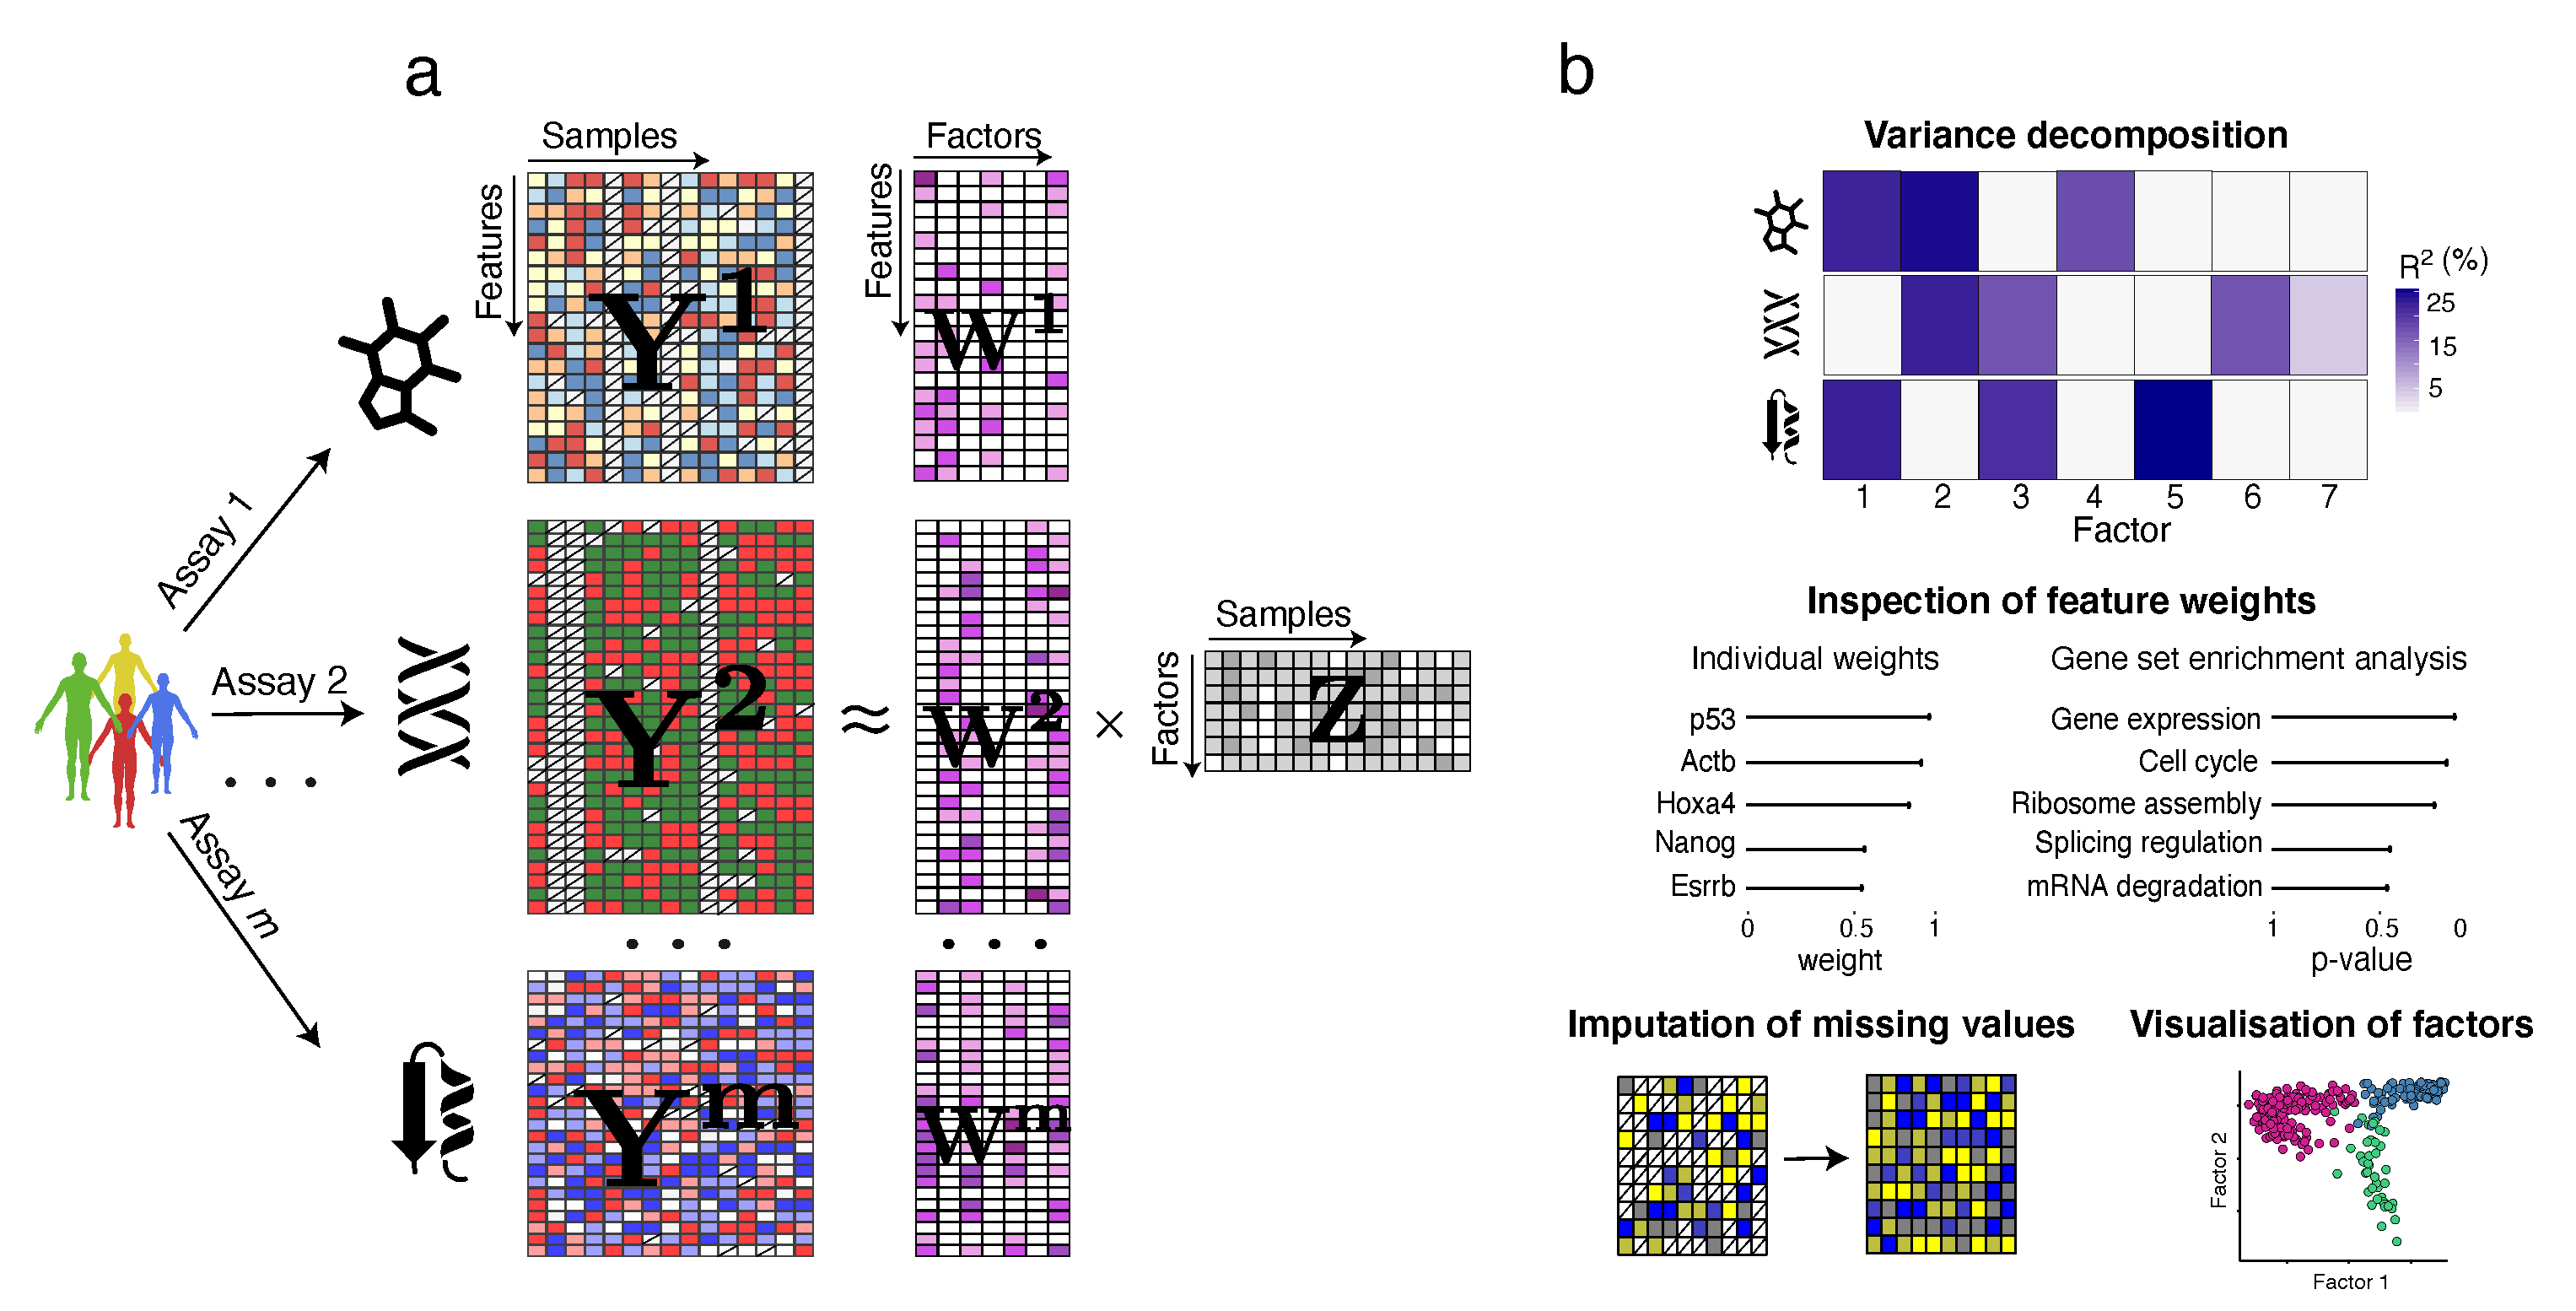
\includegraphics[width=1.0\textwidth]{MOFA}
		\caption{\textbf{MOFA overview}.\\
		The model takes $M$ data matrices as input ($\bfY^1, \cdots, \bfY^M$), one or more from each data modality, with co-occurrent samples but features that are not necessarily related and can differ in numbers. MOFA decomposes these matrices into a matrix of factors ($\bfZ$) and $M$ weight matrices, one for each data modality ($\bfW^1, \cdots, \bfW^M$). White cells in the weight matrices correspond to zeros, i.e. inactive features, whereas the cross symbol in the data matrices denotes missing values. The trained MOFA model can be queried for different downstream analyses.}
		\label{fig:MOFA}
	\end{center}
\end{figure}


\subsubsection{Inference}

To make the model scalable to large data sets we adopt a Variational inference framework with a structured mean field approximation. A detailed overview is given in \Cref{section:variational_inference}, and details on the variational updates for the MOFA model are given in Appendix~\ref{appendix:mofa}. To enable efficient inference for non-Gaussian likelihoods we employ local bounds \cite{Jaakkola2000,Seeger2012}. This is described in detail in \Cref{section:mofa_ngaussian}.


\subsection{Model selection and consistency across random initilizations} \label{section:mofa_robustness}

The optimisation problem in MOFA is not convex and the resulting posterior distributions depend on the initialisation of the model. Thus, when doing random initialisation of the parameters and/or expectations it becomes mandatory to perform model selection and assess the consistency of the factors across different trials.\\
The strategy we adopted in this work is to train several MOFA models under different parameter initialisations, where the expectation of each node is randomly sampled from its underlying distribution. After fitting, we select the model with the highest ELBO for downstream analysis. In addition, we evaluate the robustness of the factors by plotting the Pearson correlations between factors across all trials:

\begin{figure}[H]
	\centering 	
	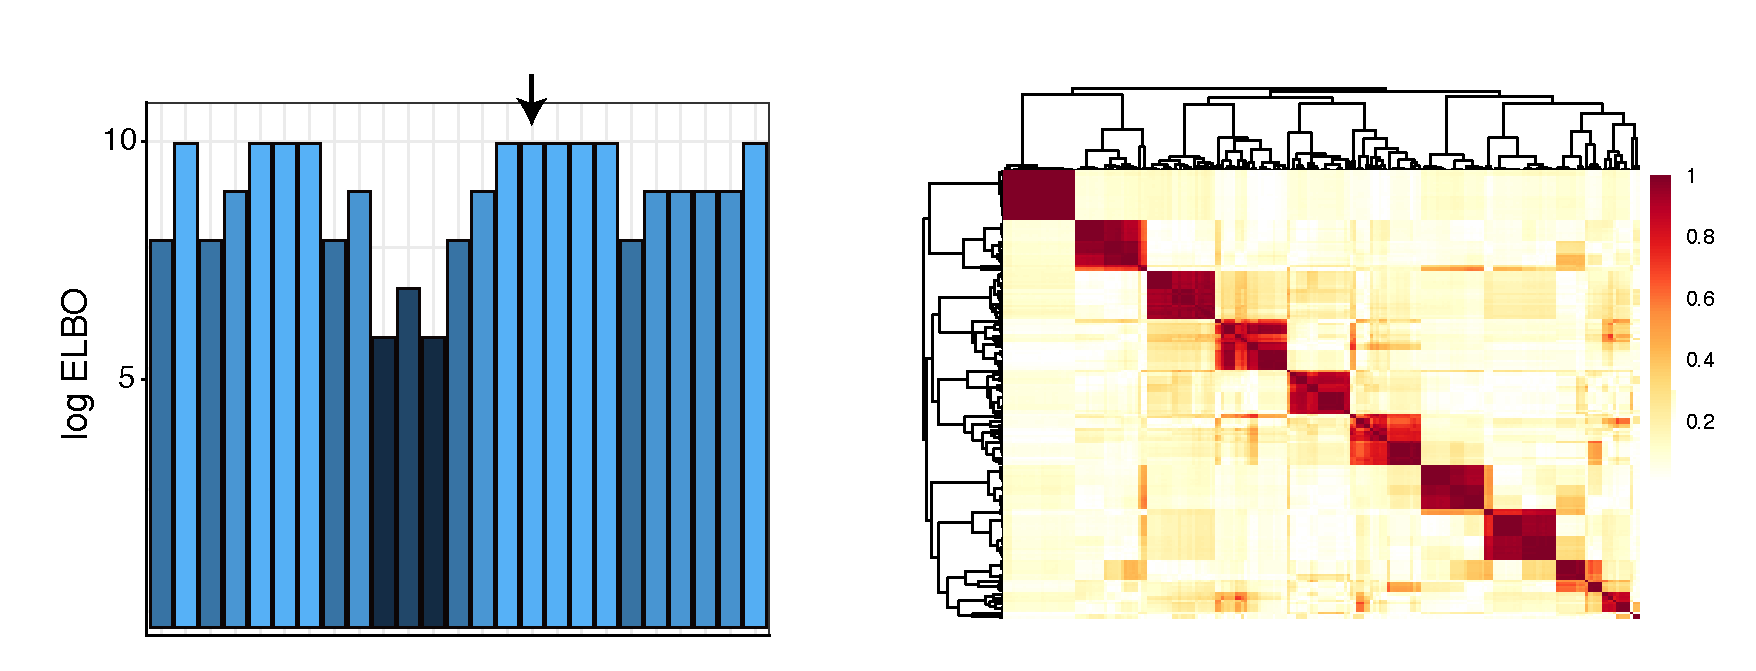
\includegraphics[width=1.0\textwidth]{MOFA_robustness}
	\caption{ \textbf{Model selection and robustness analysis in MOFA}.\\
	The left plot the log ELBO (y-axis) for 25 model instances (x-axis). The arrow indicates the model with the highest ELBO that would be selected for downstream analysis. The right plot displays the absolute value of the Pearson correlation coefficient between pairwise combinations of all factors across the 25 model instances. A block-diagonal matrix indicates that factors are robustly estimated regardless of the initialisation.}
	\label{fig:MOFA_robustness}
\end{figure}


\subsection{Learning the number of factors} \label{section:mofa_nfactors}

As described in \Cref{section:hierarchical_priors}, the use of an ARD prior allows factors to be actively pruned by the model if their variance explained is negligible. In the implementation we control the pruning of factors by a hyperparameter that defines a threshold on the minimum fraction of variance explained by a factor (across all views).\\
Additionally, because of the non-convexity of the optimisation problem, different model instances can potentially yield solutions with different number of active factors (\Cref{fig:mofa_nfactors}). Thus, the optimal number of factors can be selected by the model selection strategy outlined in \Cref{section:mofa_robustness}.

\begin{figure}[H]
	\centering 	
	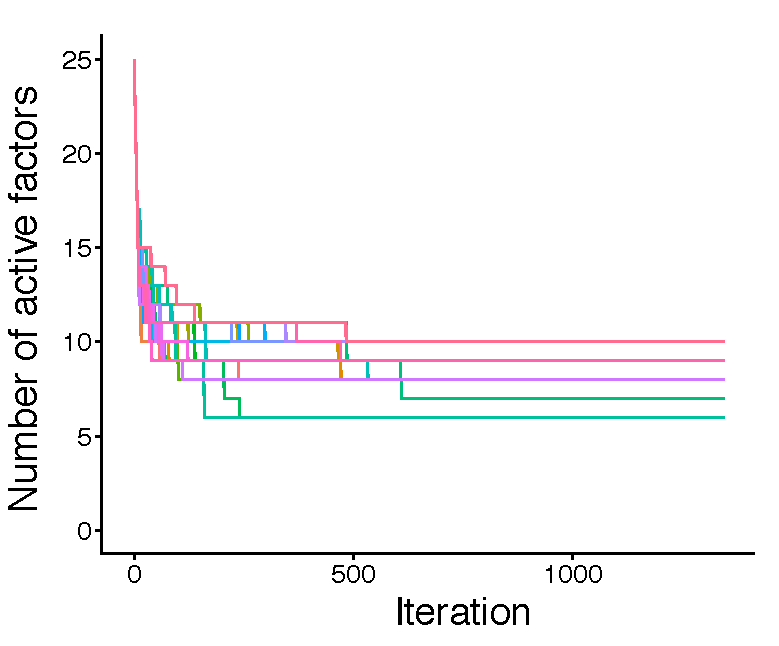
\includegraphics[width=0.6\textwidth]{MOFA_nfactors}
	\caption{\textbf{Training curve for the number of active factors across 25 different model instances}.\\
	The y-axis displays the number of active factors. The x-axis displays the iteration number. Different lines denote different model instances.}
	\label{fig:mofa_nfactors}
\end{figure}


\subsection{Monitoring convergence}

An attractive property of Variational inference is that the objective function (the ELBO) increases monotonically at every iteration. This provides a simple way of monitoring convergence:
\begin{figure}[H]
	\centering 	
	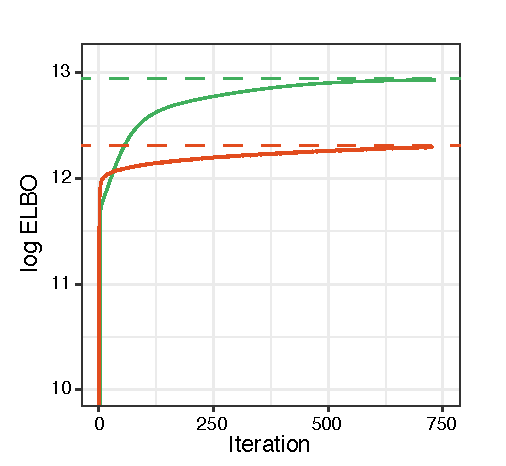
\includegraphics[width=0.5\textwidth]{elbo_convergence}
	\caption{Training curve for two diffent instances of MOFA with random initialisations. The y-axis displays the log of the ELBO, with higher values indicating a better fit. The x-axis displays the iteration number. The horizontal dash lines mark the value of the ELBO upon convergence. }
	\label{fig:elbo_convergence}
\end{figure}

Training is stopped when the change in the lower bound becomes smaller than a predefined threshold.

% COPIED
%\subsection{Guidelines for the selection of data modalities} \label{section:guidelines_views}
%Data modalities typically correspond to different molecular layers, but the user can also explore data-driven modalities that do not necessarily correspond to different molecular readouts (see for example Figure 3). Analogous to the number of samples per group, the size of the data modality can have an influence on the latent space, such that larger data modalities can contribute more to the latent space than small data modalities, simply because they have larger amounts of variation. The signal that can be extracted from small data modalities will depend on the degree of structure within the dataset, the levels of noise and on how strong the sample imbalance is between data modalities. Hence, in the case of a strong feature imbalance, we recommend the user to subset highly variable features in the large data modalities to maintain the number of features within the same order of magnitude.


\subsection{Modelling and inference with non-Gaussian data} \label{section:mofa_ngaussian}

To implement efficient variational inference in conjunction with a non-Gaussian likelihood we adapt prior work from \cite{Seeger2012} using local variational bounds. The key idea is to dynamically approximate non-Gaussian data by Gaussian pseudo-data based on a second-order Taylor expansion.  To make the approximation justifiable we need to introduce variational parameters that are adjusted alongside the updates to improve the fit.	\\
Denoting the parameters in the MOFA model as $\bfX= (\bfZ,\bfW,\balpha,\btau,\btheta)$, recall that the variational framework approximates the posterior $p(\bfX | \bfY )$ with a distribution $q(\bfX)$, which is indirectly optimised by optimising a lower bound of the log model evidence. The resulting optimization problem can be re-written as
\begin{equation*}
\min_{q(\bfX)} -\Lagr(\bfX) =  \min_{q(\bfX)} \E_q \big[ -\log p(\bfY|\bfX) \big] + \KL[q(\bfX)||p(\bfX)].
\end{equation*}

Expanding the MOFA model to non-Gaussian likelihoods we now assume a general likelihood of the form $p(\bfY|\bfX)=p(\bfY|\bfC)$ with $\bfC = \bfZ\bfW^{T}$, that we can write as
\begin{equation*}
-\log p(\bfY|\bfX) = \sum_{n=1}^{N} \sum_{d=1}^{D} f_{nd} (c_{nd})
\end{equation*}
with $f_{nd}(c_{nd}) = -\log p(y_{nd}|c_{nd})$. I dropped the index $m$ for clarity.\\
Extending \cite{Seeger2012} to our heteroscedastic noise model, we require $f_{nd}(c_{nd})$ to be twice differentiable and bounded by $\kappa_d$, such that $f_{nd}''(c_{nd}) \leq \kappa_d \,\forall n,d$. This holds true in many important models as for example the Bernoulli and Poisson likelihoods. Under this assumption a lower bound on the log likelihood can be constructed using Taylor expansion,
\begin{equation*}
f_{nd}(c_{nd}) \leq \frac{\kappa_d}{2} (c_{nd} - \zeta_{nd})^2 + f'(\zeta_{nd})(c_{nd} - \zeta_{nd}) + f_{nd}(\zeta_{nd}) := q_{nd}(c_{nd},\zeta_{nd}),
\end{equation*}
where $\bZeta =  \zeta_{nd} $ are additional variational parameters that determine the location of the Taylor expansion and have to be optimised to make the lower bound as tight as possible. Plugging the bounds into above optimization problem, we obtain:
\begin{equation*}
\min_{q(\bfX),\bZeta} \quad \sum_{d=1}^{D}\sum_{n=1}^{N} \E_q [ q_{nd}(c_{nd},\zeta_{nd})] + \KL[q(\bfX)||p(\bfX)]
\end{equation*}
The algorithm propsed in \cite{Seeger2012} then alternates between updates of $\bZeta$ and $\mathrm{q}(\bTheta)$. The update for $\bZeta$ is given by
\begin{equation*}
\zeta \leftarrow \E[\bfW]\E[\bfZ]^{T}
\end{equation*}
where the expectations are taken with respect to the corresponding $q$ distributions.\\
% In order to find the updates for $q(\bTheta)$ we bring the taylor approximation of $q(f_{nd})$ in q audratic form:
% \begin{equation*}
% q(f_{nd},\zeta_{nd}) \propto \frac{\kappa_d}{2}(f_{nd} - (zeta_{nd} - g(\zeta_{nd})/\kappa_d))^2
% \end{equation*}
% and note that this is proportional to the log of a Gaussian distribution $-log \Normal (\hat{y}_{nd}|f_{ng},\frac{1}{ng})$ where $\hat{y}_{nd} = zeta_{nd} - g'(\zeta_{nd})/\kappa_d$ is defined as a pseudodata based on the zero-inflated observations.
% Consequently, for fixed $\zeta_{nd}$, the updates of the variational distributions $Q(X)$ and $Q(W)$ are equivalent to the ones derived in X, but with pseudodata $\hat{Y}$ and precision $\kappa_g$
On the other hand, the updates for $q(\bfX)$ can be shown to be identical to the variational Bayesian updates with a conjugate Gaussian likelihood when replacing the observed data $\bfY$ by a pseudo-data $\hat{\bfY}$ and the precisions $\tau_{nd}$ (which were treated as random variables) by the constant terms $\kappa_d$ introduced above. 

The pseudodata is given by:
\begin{equation*}
\hat{y}_{nd} = \zeta_{nd} - f'(\zeta_{nd})/\kappa_d
\end{equation*}
depending on the log likelihoods $f(\cdot)$ different $\kappa_d$ are used resulting in different pseudo-data updates. Two special cases implemented in MOFA are the Poisson and Bernoulli likelihood described in the following.

\subsubsection*{Bernoulli likelihood for binary data}
When the observations are binary, $y \in \{0,1\}$, they can be modelled using a Bernoulli likelihood:
%\begin{equation*}
%p(y|c) = \frac{e^{yc}}{1+e^c}
%\end{equation*}
%The second derivative of the log likelihood is bounded by:
%\begin{equation*}
%f''(c) = \sigma(c)\sigma(-c) \leq 1/4 := \kappa
%\end{equation*}
%where $\sigma$ is the sigmoid function $f(c) = 1/(1+e^{-c})$.\\
%The pseudodata updates are given by
%\begin{equation*}
%\hat{y}_{nd} = \zeta_{nd} - 4*(\sigma(\zeta_{nd}) - y_{nd})
%\end{equation*}
\begin{equation*}
\bfY|\bfZ,\bfW \sim \text{Ber}(\sigma(\bfZ\bfW^T)),
\end{equation*} where $\sigma(a)=(1+e^{-a})^{-1}$ is the logistic link function and $\bfZ$ and $\bfW$ are the latent factors and weights in our model, respectively.\\
In order to make the variational  inference efficient and explicit as in the Gaussian case, we aim to approximate the Bernoulli data by a Gaussian pseudo-data as proposed in \cite{Seeger2012} and described above which allows to recycle all the updates from the model with Gaussian views. While \cite{Seeger2012} assumes a homoscedastic approximation with a spherical Gaussian, we adopt an approach following \cite{Jaakkola2000}, which allows for heteroscedaticity and provides a tighter bound on the Bernoulli likelihood.\\
Denoting $c_{nd}=(\bfZ\bfW^T)_{nd}$ the Jaakkola upper bound \cite{Jaakkola2000} on the negative log-likelihood is given by
\begin{align*}
\begin{split}
-\log\left(p(y_{nd}|c_{nd})\right) &= -\log\left(\sigma\left((2y_{nd}-1)  c_{nd}\right)\right)\\
& \leq -\log(\zeta_{nd})-\frac{(2y_{nd}-1)c_{nd}-\zeta_{nd})}{2} +\lambda(\zeta_{nd})\left(c_{nd}^2 -\zeta_{nd}^2 \right)\\
& =: b_J(\zeta_{nd}, c_{nd},y_{nd} )
\label{jaakkola}
\end{split}
\end{align*}
with $\lambda$ given by $\lambda(\zeta)=\frac{1}{4\zeta}\tanh\left(\frac{\zeta}{2}\right)$.\\
This can easily be derived from a first-order Taylor expansion on the function $f(x) = - \log(e^{\frac{x}{2}}+e^{-\frac{x}{2}}) = \frac{x}{2}-\log(\sigma(x))$ in $x^2$ and by the convexity of 
$f$ in $x^2$ this bound is global as discussed in \cite{Jaakkola2000}.\\
In order to make use of this tighter bound but still be able to re-use the variational updates from the Gaussian case we re-formulate the bound as a Gaussian likelihood on pseudo-data $\hat{\bfY}$.\\
As above we can plug this bound on the negative log-likelihood into the variational optimization problem to obtain  \begin{equation*}
\min_{q(\bfX),\bZeta} \quad \sum_{d=1}^{D}\sum_{n=1}^{N} \mathbb{E}_q b_J(\zeta_{nd}, c_{nd},y_{nd} ) + \KL[q(\bfX)||p(\bfX)].
\end{equation*}
This is minimized iteratively in the variational parameter $\zeta_{nd}$ and the variational distribution of Z,W:\\
Minimizing in the variational parameter $\zeta$ this leads to the updates given by
\begin{equation*}
	\zeta_{nd}^2 = \mathbb{E}[c_{nd}^2]
\end{equation*}
as described in \cite{Jaakkola2000}, \cite{Bishop2006}.\\
For the variational distribution $q(\bfZ,\bfW)$ we observe that the Jaakkola bound can be re-written as 
\begin{equation*}
	b_J(\zeta_{nd}, c_{nd},y_{nd} ) = -\log\left(\varphi\left(\hat{y}_{nd}; c_{nd}, \frac{1}{2\lambda(\zeta_{nd})}\right)\right) + \gamma(\zeta_{nd}),
\end{equation*}
where $\varphi(\cdot; \mu, \sigma^2)$ denotes the density function of a normal distribution with mean $\mu$ and variance $\sigma^2$ and $\gamma$ is a term only depending on $\bZeta$. This allows us to re-use the updates for $\bfZ$ and $\bfW$ from a setting with Gaussian likelihood by considering the Gaussian pseudo-data 
\begin{equation*}
	\hat{y}_{nd}= \frac{2y_{nd}-1}{4 \lambda(\zeta_{nd})}
\end{equation*}
updating the data precision as $\tau_{nd} = 2\lambda(\zeta_{nd})$ using  updates generalized for sample- and feature-wise precision parameters on the data.


\subsubsection*{Poisson likelihood for count data}

When observations are a natural numbers, such as count data $y \in \N = \{0,1,\cdots\}$, they can be modelled using a Poisson likelihood:
\begin{equation*}
	p(y|c) = \lambda(c)^y e^{-\lambda(c)}
\end{equation*}
where $\lambda(c)>0$ is the rate function and has to be convex and log-concave in order to ensure that the likelihood is log-concave.\\
As done in \cite{Seeger2012}, here we choose the following rate function: $\lambda(c)=\log(1+e^c)$.

Then an upper bound of the second derivative of the log-likelihood is given by
\begin{equation*}
	f''_{nd}(c_{nd}) \leq \kappa_d = 1/4 + 0.17*\max(\bfy_{:,d}).
\end{equation*}
%The bound degrades with the presence of entries with large values. Thus, we follow common practice and clip overly large counts.\\
The pseudodata updates are given by
\begin{equation*}
	\hat{y}_{nd} = \zeta_{nd} - \frac{\mathrm{S}(\zeta_{nd})(1-y_{nd}/\lambda(\zeta_{nd}))}{\kappa_d}.
\end{equation*}

\pagebreak
	 
\subsection{Theoretical comparison with published methods}

A variety of latent variable models exist with the aim of perfoming multi-view data integration, most of them inspired by the Group Factor Analysis formulation. A summary is provided in the table below. MOFA is the only method that scales to large data sets (employs Variational Bayes inference instead of MCMC-based approaches), has a combination of ARD and spike-slab regularisation on the weights, and is also capable of handling non-gaussian modalities and missing values.

\begin{table}[H]
	\begin{tabular}{@{}lllllll} 
		\toprule
		{\textbf{Publication}} & {\textbf{Inference}} & {\textbf{\parbox{2.1cm}{View-wise\\ sparsity}}} & {\textbf{\parbox{2.4cm}{Feature-wise\\ sparsity}}} & {\textbf{\parbox{1.3cm}{Missing\\ values}}} & {\textbf{Likelihood}} &  \parbox{1.5cm}{{\textbf{Noise\\ model}}} \\ \toprule
		\parbox{2.2cm}{Shen2009} & \parbox{2.1cm}{EM,\\ grid search} & \parbox{2.1cm}{$L_1$- penalties} & $L_1$-penalty & No & Gaussian & \parbox{1.5cm}{Hetero-\\scedastic} \\\midrule
		\parbox{2.2cm}{Mo2013} &  \parbox{2.1cm}{EM,\\ grid search} & \parbox{2.1cm}{$L_1$- penalties} & $L_1$-penalty & No &\parbox{2cm}{Gaussian,\\Poisson,\\Bernoulli}  & \parbox{1.5cm}{Hetero-\\scedastic} \\\midrule
		\parbox{2.2cm}{Virtanen2012} & VB & ARD & None & No & Gaussian & \parbox{1.5cm}{Homo-\\scedastic} \\\midrule
		\parbox{2cm}{Klami2014} & VB & ARD & None & No & Gaussian & \parbox{1.5cm}{Homo-\\scedastic} \\ \midrule
		\parbox{2cm}{Bunte2016}  & Gibbs & ARD & Spike-Slab & No & Gaussian & \parbox{1.5cm}{Homo-\\scedastic} \\ \midrule
		\parbox{2cm}{Hore2016}  & VB  & None & Spike-Slab & Yes  & Gaussian & \parbox{1.5cm}{Hetero-\\scedastic}  \\ \midrule
		\parbox{2cm}{Remes2016}  & VB & ARD & None & No & Gaussian & \parbox{1.5cm}{Homo-\\scedastic} \\ \midrule
		\parbox{1.7cm}{Zhao2015} & Gibbs & ARD & \parbox{2.5cm}{Three-parameter\\ beta prior} & No & Gaussian & \parbox{1.5cm}{Hetero-\\scedastic} 
		\\ \midrule
		\parbox{2.6cm}{{Leppaaho2017},\\ {2017}}  & {Gibbs} & {ARD} & {Spike-Slab} & {Yes} & {Gaussian} & \parbox{2cm}{{Homo-}\\{scedastic}} \\ \midrule
		MOFA  & VB & ARD & Spike-Slab & Yes & \parbox{2cm}{Gaussian,\\Poisson,\\Bernoulli} & \parbox{2cm}{Hetero-\\scedastic} \\  \bottomrule
	\end{tabular}
	\caption{\textbf{Overview of latent variable methods for multi-view data integration.} Abbreviations used: VB (variational Bayes inference), Gibbs (Gibbs sampling based inference), ARD(Automatic Relevance Determination)}
	\label{GFAtable}
								
\end{table}

